\section{Comportamento Caratteristico del Modello a Taglia Finita}\label{Parte A}
A questo punto si hanno tutti gli elementi per studiare le caratteristiche del sistema di Ising attraverso la simulazione computazionale.
Ricapitolando, i principali osservabili che è possibile definire sui microstati $\phi=\lbrace \ldots, \sigma_{i\, j} ,\ldots\rbrace$ del sistema sono due:
\begin{itemize}
\item \underline{Spin Totale} $$S= \sum_{i,j=0}^{L}\sigma_{i\, j}$$
\item \underline{Energia Totale} $$ E = H(\phi) = \sum_{i,j=0}^{L}\biggr(\sigma_{i\, j}\big(\sigma_{(i+1)\, j} + \sigma_{i\, (j+1)}\big)\biggr)$$.
\end{itemize}
dove $L$ corrisponde al numero di spin in una riga, $N=L^2$ e $\sigma_{i\, j}$ e la matrice degli spin.
\newline
Le osservabili macroscopiche sono invece quattro, il loro valore d'aspettazione è da calcolare come valore medio delle "osservabili istantanee" valutate sulle singole configurazioni della catena di Markov-Montecarlo $(\phi_1,\ldots,\phi_k)$ :
\begin{itemize}
\item \underline{Magnetizzazione Media} $$\langle|M|\rangle= \langle\dfrac{|S|}{N}\rangle$$
\item \underline{Densità di Energia Interna Media} $$\langle H \rangle = \langle \dfrac{E}{N} \rangle $$
\item \underline{Calore Specifico} $$c = \beta^2 N \biggr( \langle H^2 \rangle - \langle H\rangle ^2 \biggr)$$
\item \underline{Suscettività Magnetica} $$\chi = \beta N \biggr( \langle M^2 \rangle - \langle M \rangle^2\biggr)$$
\end{itemize}
dove, per un generico osservabile istantaneo $O$ e per la generica catena $ (\phi_1, \ldots, \phi_K)$ di configurazioni campionate, vale che
\begin{displaymath}
	\langle O \rangle = \sum_{i=1}^K \dfrac{O(\phi_i)}{K}
\end{displaymath}

 \begin {figure}[h!p]
    \begin{center}
	\caption[1) ParteA\_MvsBeta.cpp \quad $/\;$ 2) ParteA\_HvsBeta.cpp ]{Magnetizzazione Assoluta e Densità di Energia}\label{fig: MvsBeta}
        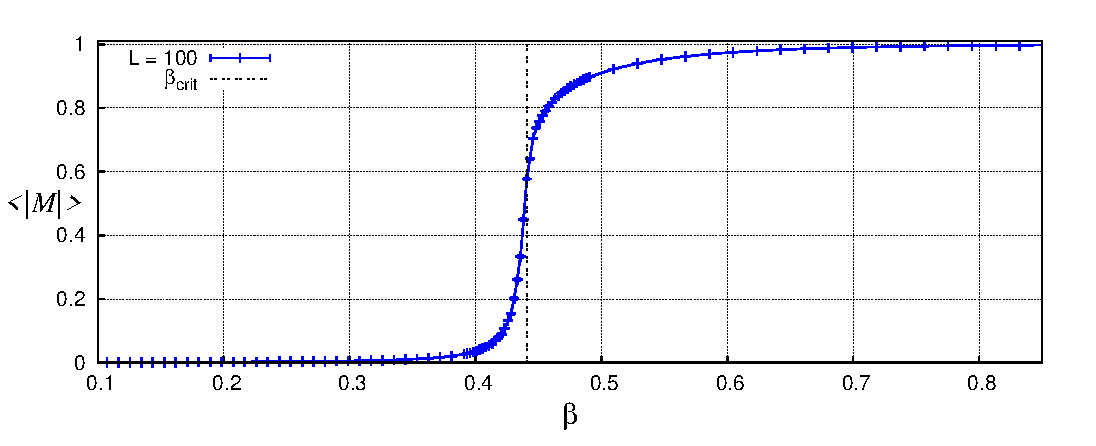
\includegraphics[scale=0.8]{Immagini/ParteA/MvsBeta}
     \newline
        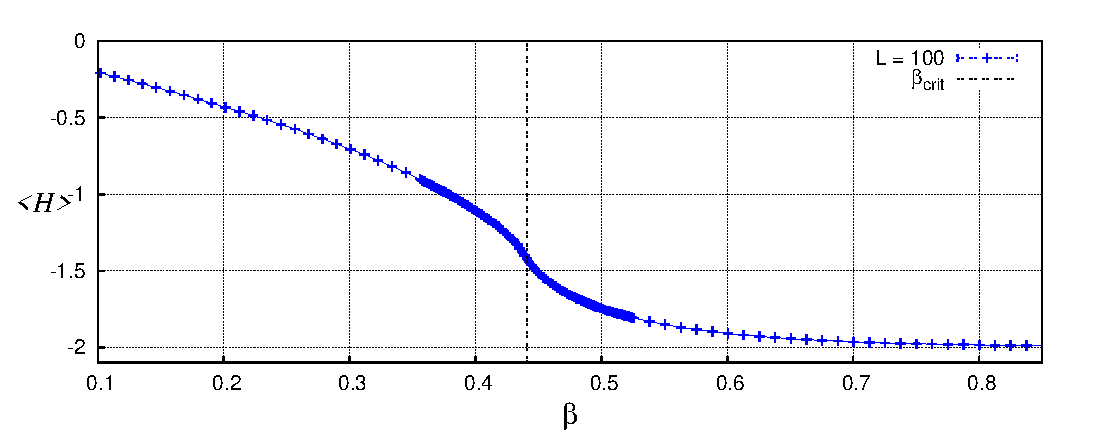
\includegraphics[scale=0.8]{Immagini/ParteA/HvsBeta}
     \newline   
	    \footnotesize L=100, $K_{metro} = 15000$, $K_{cluster} = 1500$  
    \end{center}
 \end {figure} 
 \begin {figure}[h!p]
    \begin{center}
	\caption[1) ParteA\_ChivsBeta.cpp \quad $/\;$ 2)  ParteA\_cvsBeta.cpp ]{Suscettività Magnetica e Capacità Termica}\label{fig: ChivsBeta}
        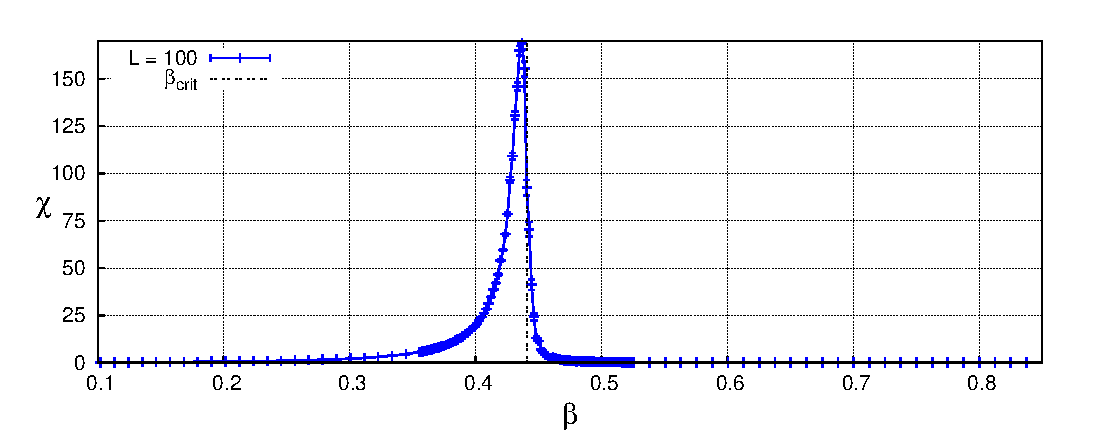
\includegraphics[scale=0.8]{Immagini/ParteA/ChivsBeta}
     \newline    
        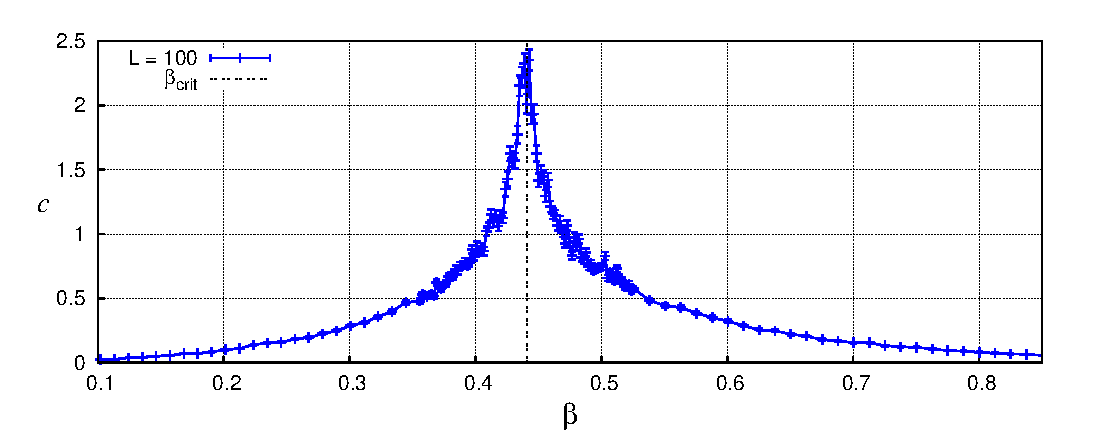
\includegraphics[scale=0.8]{Immagini/ParteA/cvsBeta}
     \newline   
		\footnotesize L=100, $K_{cluster} = 1500$  
    \end{center}
 \end {figure}

Stampando l'andamento di questi osservabili al variare della temperatura $\beta$ (figure \ref{fig: MvsBeta} e \ref{fig: ChivsBeta}) si osserva immediatamente la peculiarità del modello di Ising, ovvero la presenza di una transizione di fase attorno alla Temperatura Critica, prevista teoricamente al valore:
$$T_c =   \dfrac{\log( 1 +\sqrt{2})}{2}  = 0.44068$$
presente non sono al limite termodinamico ma anche per $L$ finito. 

\clearpage
\subsection{Calcolo dell'errore}
Le barre dell'errore nei grafici precedenti sono state calcolate tramite l'algoritmo di \emph{Jack-Knife}.
Nelle figure (\ref{fig: SigmaMvsBeta}) è mostrato l'andamento dell'incertezza per gli osservabili $M$ e $H$ calcolato tramite l'algoritmo precedente e tramite l'algoritmo di \emph{Binning} indicato per la stima dell'errore in presenza di misure correlate.

 \begin {figure}[h!]
    \begin{center}
	\caption[1) ParteA\_SigmaMvsBeta.cpp \quad $/\;$ 2) ParteA\_SigmaHvsBeta.cpp ]{Calcolo dell'incertezza sui valori d'aspettazione di $M$ e $H$ (\footnotesize vari algoritmi)}\label{fig: SigmaMvsBeta}
        \includegraphics[scale=1]{Immagini/ParteA/SigmaMvsBeta}
     \newline    
        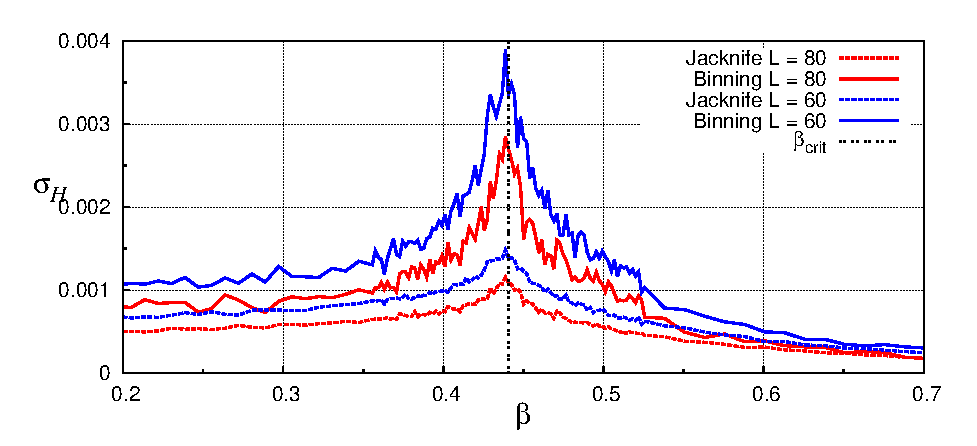
\includegraphics[scale=1]{Immagini/ParteA/SigmaHvsBeta}
     \newline   
		\footnotesize $K_{cluster} = K_{metro} = 1500$, $bin = 12$  
    \end{center}
 \end {figure}
I grafici ottenuti hanno forma simile a quelli per $\chi$ e $c$, la cosa non sorprende essendo tali osservabili legati ,  per definizione, alla varianza della magnetizzazione e dell'energia. Si nota inoltre che l'algoritmo usato porta ad una generica sottostima dell'errore rispetto al algoritmo di Binning, ma è stato scelto comunque per la maggiore semplicità di implementazione.
\newline
La crescita dell'incertezza in prossimità della temperatura critica e la sua dipendenza dalla taglia, sono l'effetto della maggiore dispersione attorno al valore medio a cui sono sottoposti gli osservabili $H$ e $M$ in queste condizioni.
 
 \begin {figure}[h!]
    \begin{center}
	\caption[1) ParteA\_distroM.cpp $\rightarrow$ distroM\_file.p \quad $/\;$ 2) ParteA\_distroH.cpp $\rightarrow$ distroH\_file.p ]{Distribuzione di probabilità sui valori d'aspettazione di $M$ e $H$ (\footnotesize vari algoritmi)}\label{fig: DistroM}
        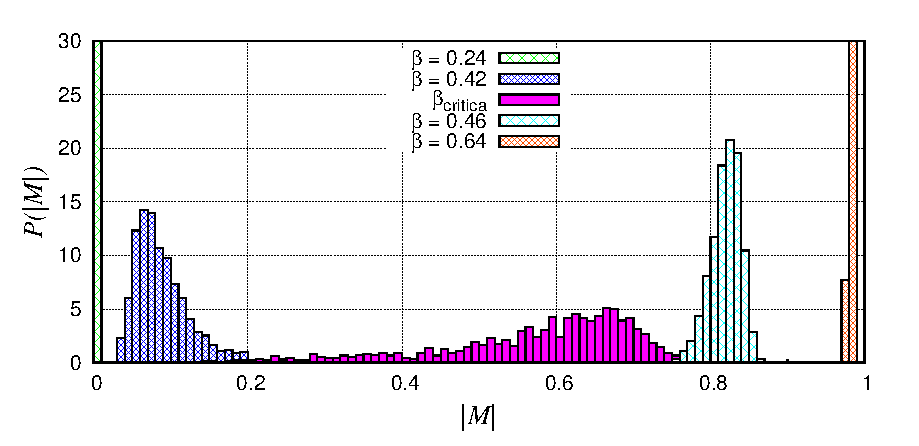
\includegraphics[scale=1]{Immagini/ParteA/distroM}
     \newline    
        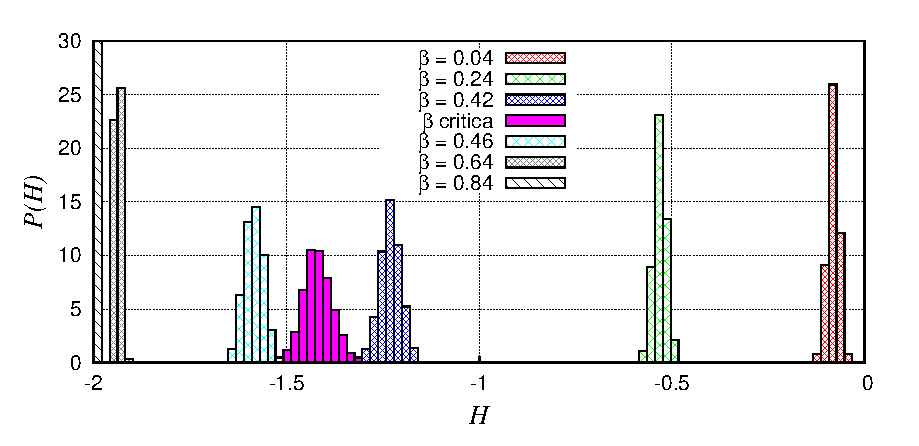
\includegraphics[scale=1]{Immagini/ParteA/distroH}
     \newline   
		\footnotesize $K_{cluster}$ \newline(nb: Nel grafico il range dell'asse è tagliato per rendere più visibili le distribuzioni vicino a $T_c$, lontano da $T_c$ le distribuzioni sono piccate in una sola colonna).   
    \end{center}
 \end {figure}
A prova di questo nelle figura \ref{fig: DistroM} sono mostrate le distribuzioni di probabilità( istogrammi normallizati) dei valori di $H$ e $M$ per differenti temperature di termalizzazione.